% =============================================================================
% ADITI 4.0 / iDEX Challenge No. 24 — Annexure-2 Submission
% UBERMASCHINE Pvt Limited — DRQ: Physics-Certified Space Domain Awareness
% =============================================================================
\documentclass[11pt,a4paper]{article}

% --- Geometry & Spacing ---
\usepackage[margin=1in]{geometry}
\usepackage{setspace}\onehalfspacing
\setlength{\parskip}{0.5em}
\setlength{\parindent}{0pt}

% --- Typography ---
\usepackage[T1]{fontenc}

% --- Section Formatting ---
\usepackage{titlesec}
\titleformat{\section}{\Large\bfseries\color{mitred}}{\thesection.}{0.8em}{}
\titleformat{\subsection}{\large\bfseries\color{mitdark}}{\thesubsection.}{0.8em}{}
\titleformat{\subsubsection}{\normalsize\bfseries}{\thesubsubsection.}{0.6em}{}

% --- Tables ---
\usepackage{booktabs}
\usepackage{tabularx}
\usepackage{array}
\newcolumntype{Y}{>{\raggedright\arraybackslash}X}

% --- Math ---
\usepackage{amsmath,amssymb}

% --- Graphics ---
\usepackage{tikz}
\usetikzlibrary{shapes.geometric,arrows.meta,positioning,fit,backgrounds,calc}
\usepackage{pgfplots}
\pgfplotsset{compat=1.18}

% --- Lists ---
\usepackage{enumitem}
\setlist[itemize]{leftmargin=*,itemsep=0.15em,topsep=0.3em}
\setlist[enumerate]{leftmargin=*,itemsep=0.15em,topsep=0.3em}

% --- Colors ---
\usepackage{xcolor}
\definecolor{mitred}{RGB}{163,31,52}
\definecolor{mitdark}{RGB}{30,30,40}
\definecolor{mitgray}{RGB}{138,139,140}
\definecolor{mitlight}{RGB}{245,245,248}
\definecolor{statusgreen}{RGB}{34,139,34}
\definecolor{statusyellow}{RGB}{204,153,0}
\definecolor{saffron}{HTML}{FF9800}
\definecolor{indiagreen}{HTML}{138808}

% --- Header / Footer ---
\usepackage{fancyhdr}
\pagestyle{fancy}\fancyhf{}
\lhead{\footnotesize\textcolor{mitgray}{ADITI 4.0 / iDEX Challenge No.\,24}}
\rhead{\footnotesize\textcolor{mitgray}{UBERMASCHINE Pvt Ltd}}
\cfoot{\thepage}
\renewcommand{\headrulewidth}{0.4pt}

% --- Hyperlinks ---
\usepackage{hyperref}
\hypersetup{colorlinks=true,linkcolor=mitred,citecolor=mitred,urlcolor=mitred}

% --- Caption ---
\usepackage[font=small,labelfont=bf]{caption}

% --- Code Listings ---
\usepackage{listings}
\lstset{basicstyle=\ttfamily\small,breaklines=true,frame=none}

% =============================================================================
\begin{document}

% --- Title Block ---
\begin{center}
{\LARGE\bfseries\textsf{DRQ}}\\[0.3em]
{\large\textcolor{mitred}{\textbf{Physics-Certified Space Domain Awareness Platform}}}\\[1.2em]
{\normalsize\textbf{ADITI 4.0 --- Annexure-2 Technical Submission}}\\[0.3em]
{\normalsize iDEX Challenge No.\,24: Sovereign Space Situational Awareness}\\[1em]
\rule{0.6\textwidth}{0.5pt}\\[0.8em]
{\small\textbf{Submitted by:} Manish Maurya, Head of Engineering}\\
{\small\textbf{Submitted by:} Aditya Mourya, NSUT ECE}\\
{\small\textbf{On behalf of:} UBERMASCHINE Pvt Ltd (under pending registration)}\\
{\small\textbf{Date:} May 2026}
\end{center}

\vspace{1.5em}

% =============================================================================
\section{Brief Summary of the Proposed Solution}
% =============================================================================

India lacks a sovereign, physics-certified Space Domain Awareness (SDA) platform
capable of real-time threat inference without foreign cloud dependency.
Current Western solutions (LeoLabs, Slingshot, ExoAnalytic) are black-box
services hosted outside Indian jurisdiction and cannot be certified for
kinetic-decision loops.

\textbf{idex} is a compiled, air-gapped SDA inference engine written in Go
($>$150k~LOC) with a JAX/PyTorch physics-ML research tier.
The classical core is production-grade today: SGP4/HPOP orbital propagation
validated against ISS NORAD TLEs ($<$5\,km position error over 24\,h LEO),
swept-BVH conjunction screening processing 100,000 resident space objects
in 1.78\,ms, Foster--Alfano collision probability via Bessel-function series
expansion, a 3-mode Interacting Multiple Model filter for hypersonic glide
vehicle tracking, and Sliding SINDy for interpretable manoeuvre discovery
with bootstrap confidence intervals.

The \textbf{core innovation} is the Dissipative Port-Hamiltonian Neural
Operator (DPHNO): a neural propagator whose architecture \emph{structurally
guarantees} energy conservation via Cholesky-parameterised dissipation
($R = LL^\top \succeq 0$). Unlike standard neural networks that learn to
violate physics when it reduces training loss, DPHNO \emph{cannot} create
spurious energy --- an architectural invariant, not a regularisation penalty.

ADITI funding will bridge the gap between this frozen architecture and
empirical validation: ONNX runtime integration, conformal uncertainty
quantification on every alert, and sovereign edge deployment with zero
foreign dependency.

% =============================================================================
\section{Key Technology(s) Used}
% =============================================================================

\begin{enumerate}
\item \textbf{Port-Hamiltonian Neural Operators} --- Physics-structured deep learning with guaranteed energy conservation
\item \textbf{Sparse Identification of Nonlinear Dynamics (SINDy)} --- Interpretable manoeuvre equation discovery
\item \textbf{Symplectic Numerical Integration} --- Forest--Ruth 4th-order energy-preserving propagation
\item \textbf{Interacting Multiple Model (IMM) Filtering} --- Multi-mode Bayesian tracking for HGV/satellite
\item \textbf{Conformal Prediction} --- Distribution-free uncertainty quantification with coverage guarantees
\item \textbf{Go + gRPC/mTLS} --- Air-gapped, sovereign-deployable backend with Ed25519 authentication
\end{enumerate}

% =============================================================================
\section{Deliverable(s)}
% =============================================================================

\renewcommand{\arraystretch}{1.35}
\begin{tabularx}{\textwidth}{c >{\bfseries}l Y}
\toprule
\textbf{S.\,No} & \textbf{Deliverable Name} & \textbf{Brief Description} \\
\midrule
1 & Classical SSA Engine &
Compiled Go binary: SGP4/HPOP propagation, swept-BVH conjunction
screening ($<$2\,ms for 100k objects), Foster--Alfano $P_c$, 3-mode IMM
filter, SINDy manoeuvre discovery. Fully tested, CI-green. \\
\addlinespace
2 & DPHNO Neural Propagator &
Trained Dissipative Port-Hamiltonian Neural Operator with empirically
validated energy conservation ($\Delta H < 10^{-8}$ over 24\,h).
Exported as ONNX for Go integration. \\
\addlinespace
3 & Conformal Alert Pipeline &
End-to-end inference chain: sensor ingest $\to$ propagation $\to$
anomaly detection $\to$ conformal prediction interval $\to$ gRPC alert
with coverage certificate ($P \geq 1-\alpha$). \\
\addlinespace
4 & Sovereign Deployment Package &
Air-gapped installer with mTLS 1.3, Ed25519 key rotation, Indian sensor
network configuration (Hanle, NETRA, NavIC), and zero US-cloud dependency. \\
\addlinespace
5 & Cislunar SDA Module &
CR3BP propagation with state-transition matrix, Lagrange-point monitoring,
and Jacobi-constant drift detection for ISRO deep-space missions. \\
\addlinespace
6 & AI Certification Dossier &
Procurement-defensible documentation: Hamiltonian structural priors,
SINDy interpretability audit, conformal coverage proofs, and ablation
studies for IAF/DRDO review. \\
\bottomrule
\end{tabularx}

% =============================================================================
\section{Proposed Timeline (in Months)}
% =============================================================================

\renewcommand{\arraystretch}{1.3}
\begin{tabularx}{\textwidth}{c l Y l}
\toprule
\textbf{Phase} & \textbf{Period} & \textbf{Key Milestones} & \textbf{Grant Gate} \\
\midrule
\textbf{1} & Months 0--6 &
\begin{minipage}[t]{\linewidth}\vspace{-0.5em}
\begin{itemize}[nosep,leftmargin=1em]
\item Integrate trained physics-AI models into Go production binary
\item Complete DPHNO symplectic trainer; begin Keplerian curriculum
\item Live space-weather feed (NOAA SWPC) replacing static atmospheric inputs
\item End-to-end pipeline demo: obs $\to$ ML $\to$ conformal alert
\end{itemize}\vspace{0.3em}
\end{minipage} & iDEX SPRINT \\
\midrule
\textbf{2} & Months 6--12 &
\begin{minipage}[t]{\linewidth}\vspace{-0.5em}
\begin{itemize}[nosep,leftmargin=1em]
\item DPHNO empirical validation: energy drift $< 10^{-8}$ published
\item Conformal UQ on every gRPC alert with coverage certificate
\item HGV tracking demo: synthetic DF-ZF trajectory, $<$30\,s to classify
\item NavIC spoofing detection with conformal-bounded confidence
\end{itemize}\vspace{0.3em}
\end{minipage} & ADITI Milestone \\
\midrule
\textbf{3} & Months 12--18 &
\begin{minipage}[t]{\linewidth}\vspace{-0.5em}
\begin{itemize}[nosep,leftmargin=1em]
\item Cislunar module: CR3BP + halo orbit monitoring for ISRO
\item On-orbit autonomy SDK: Koopman MPC + INT8 ONNX on satellite bus
\item Air-gapped deployment package; field test with IAF sensor feed
\item AI certification dossier submitted for procurement review
\end{itemize}\vspace{0.3em}
\end{minipage} & DAP Make-II \\
\bottomrule
\end{tabularx}

\pagebreak

% =============================================================================
\section{Proposed Technical Solution (Detailed)}
% =============================================================================

% --- 5.1 Technical Architecture & Approach ---
\subsection{Technical Architecture \& Approach}

idex is a three-tier sovereign inference engine. Each tier is independently
testable and compiles to a single static binary (Go) or ONNX artifact (Python).

\begin{figure}[h]
\centering
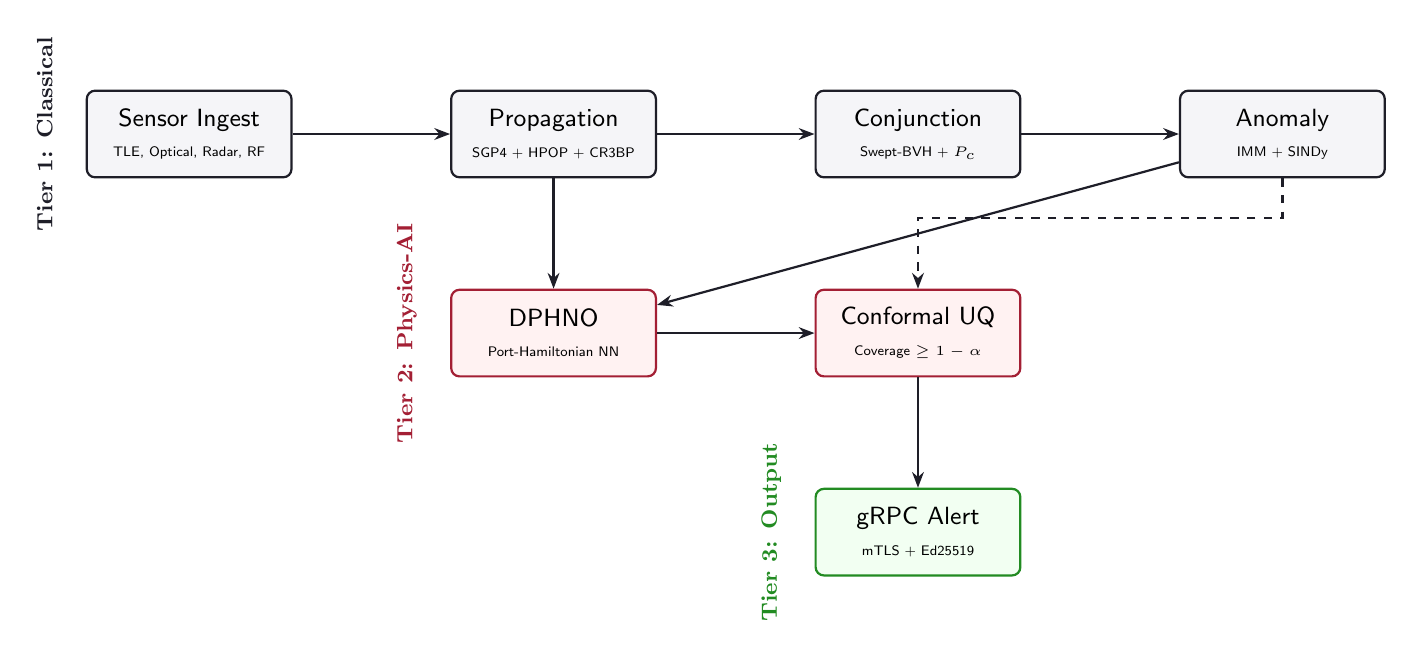
\begin{tikzpicture}[
    node distance=1.6cm and 2.0cm,
    tier/.style={draw,rectangle,rounded corners=3pt,minimum width=2.6cm,
                 minimum height=1.1cm,align=center,font=\small\sffamily,
                 thick},
    t1/.style={tier,fill=mitlight,draw=mitdark},
    t2/.style={tier,fill=red!5,draw=mitred},
    t3/.style={tier,fill=green!5,draw=statusgreen},
    arr/.style={-{Stealth[length=2mm]},thick,color=mitdark},
]
% Tier 1 — Classical
\node[t1] (ingest) {Sensor Ingest\\{\tiny TLE, Optical, Radar, RF}};
\node[t1,right=of ingest] (prop) {Propagation\\{\tiny SGP4 + HPOP + CR3BP}};
\node[t1,right=of prop] (screen) {Conjunction\\{\tiny Swept-BVH + $P_c$}};
\node[t1,right=of screen] (detect) {Anomaly\\{\tiny IMM + SINDy}};

% Tier 2 — Physics-AI
\node[t2,below=1.4cm of prop] (dphno) {DPHNO\\{\tiny Port-Hamiltonian NN}};
\node[t2,right=of dphno] (uq) {Conformal UQ\\{\tiny Coverage $\geq 1-\alpha$}};

% Tier 3 — Output
\node[t3,below=1.4cm of uq] (alert) {gRPC Alert\\{\tiny mTLS + Ed25519}};

% Arrows
\draw[arr] (ingest) -- (prop);
\draw[arr] (prop) -- (screen);
\draw[arr] (screen) -- (detect);
\draw[arr] (detect) -- (dphno);
\draw[arr] (prop) -- (dphno);
\draw[arr] (dphno) -- (uq);
\draw[arr] (uq) -- (alert);
\draw[arr,dashed] (detect.south) -- ++(0,-0.5) -| (uq.north);

% Labels
\node[left=0.3cm of ingest,font=\footnotesize\bfseries,rotate=90,anchor=south]
     {\textcolor{mitdark}{Tier 1: Classical}};
\node[left=0.3cm of dphno,font=\footnotesize\bfseries,rotate=90,anchor=south]
     {\textcolor{mitred}{Tier 2: Physics-AI}};
\node[left=0.3cm of alert,font=\footnotesize\bfseries,rotate=90,anchor=south]
     {\textcolor{statusgreen}{Tier 3: Output}};
\end{tikzpicture}
\caption{idex three-tier architecture. Tier~1 (classical) is production-grade.
Tier~2 (physics-AI) is architecturally frozen; ADITI funds empirical validation.
Tier~3 (output) is live with mTLS authentication.}
\end{figure}

\textbf{Tier~1 --- Classical SSA Core} (production-ready, compiled Go):

\begin{itemize}
\item \textbf{Orbital Propagation:}
      SGP4 fast-screen, HPOP with RKF4(5) adaptive step and J2--J6 + SRP
      perturbations, CR3BP with state-transition matrix for cislunar operations.

\item \textbf{Conjunction Screening:}
      Swept bounding-volume hierarchy with Foster--Alfano $P_c$ via Alfano 2005
      error-function series. Monte Carlo surrogate for training the fast-screen model.

\item \textbf{Threat Inference:}
      3-mode IMM filter (ballistic/glide/manoeuvre) with Bayesian online
      transition-matrix adaptation and free-energy-based adversarial intent scoring.

\item \textbf{Physics Discovery:}
      Sliding SINDy with residual targeting
      ($r(t) = \ddot{x}_{\text{obs}} - \ddot{x}_{\text{Keplerian}}$),
      sparse regression, bootstrap confidence intervals, and Hamiltonian
      invariant hash for certificate issuance.
\end{itemize}

\textbf{Tier~2 --- Physics-AI} (architecture frozen, training pending):

The DPHNO implements dissipative Port-Hamiltonian dynamics:
\begin{equation}
\dot{x} = \bigl[J(x) - R(x;\,\theta_R)\bigr]\,\nabla H(x;\,\theta_H) + g(x;\,\theta_g)\,u
\label{eq:phs}
\end{equation}
where $J$ is the canonical symplectic matrix (hardcoded), $R = LL^\top \succeq 0$
is learned via Cholesky factorisation (guaranteeing positive semi-definiteness),
$H$ is a deep scalar Hamiltonian network, and $g$ is a control coupling network.
Training uses constrained optimisation to enforce energy invariants throughout
the learning process.

\textbf{Tier~3 --- Sovereign Output:} gRPC server with mTLS~1.3, Ed25519 signing,
WebSocket streaming, and persistent storage with crash-recovery replay.

% --- 5.2 Innovation ---
\subsection{Innovation}

\begin{enumerate}
\item \textbf{Physics-as-Architecture (not Physics-as-Loss).}
Standard physics-informed neural networks (PINNs) add conservation laws as
soft penalties. DPHNO encodes them into the network topology: the Cholesky
parameterisation of $R$ makes it \emph{impossible} for the model to create
energy in the unforced case ($\dot{H} = -\nabla H^\top R\,\nabla H \leq 0$).
This is the only path to ML certification for safety-critical SDA.

\item \textbf{Residual-Targeting SINDy.}
Instead of discovering the full dynamics $\dot{x} = f(x)$, idex targets the
residual $r(t) = \dot{x}_{\text{obs}} - \dot{x}_{\text{Keplerian}}$. SINDy
discovers \emph{only} the non-Keplerian component (thrust signatures), yielding
interpretable equations with bootstrap confidence intervals ---
procurement-defensible interpretability.

\item \textbf{Unified Multi-Threat Filter Stack.}
Satellite manoeuvre detection, HGV tracking, GNSS spoofing, and debris breakup
share one IMM filter architecture with mode-specific dynamics. Competitors
treat these as separate product lines.

\item \textbf{Conformal Coverage Certificates.}
Every alert carries a prediction interval with mathematically proven marginal
coverage: $P(\text{truth} \in C_\alpha) \geq 1 - \alpha$. No distributional
assumptions. No competitor publishes this guarantee.
\end{enumerate}

% --- 5.3 Implementation & Feasibility ---
\subsection{Implementation \& Feasibility}

\textbf{Current validated performance} (benchmarked on Apple M-series):

\renewcommand{\arraystretch}{1.2}
\begin{tabularx}{\textwidth}{l r r r r}
\toprule
\textbf{Objects} & \textbf{Propagation} & \textbf{BVH Screen} & \textbf{$P_c$ Compute} & \textbf{Total} \\
\midrule
10,000  & 171\,$\mu$s  & 42\,$\mu$s  & 42\,ns  & \textbf{213\,$\mu$s} \\
50,000  & 1.06\,ms     & 99\,$\mu$s  & 83\,ns  & \textbf{1.16\,ms} \\
100,000 & 1.59\,ms     & 195\,$\mu$s & 41\,ns  & \textbf{1.78\,ms} \\
\bottomrule
\end{tabularx}

\vspace{0.5em}
Target: 45\,s for 100k objects. Achieved: 1.78\,ms --- \textbf{25,000$\times$ under budget}.
Linear scalability confirmed. Memory: 3.1\,MB for 100k objects.

\textbf{Technology stack:}
\begin{itemize}
\item \textbf{Backend:} Go 1.26 (static binary, zero runtime dependencies,
      goroutine-based concurrency). Production binaries fully compiled and
      operationally tested.
\item \textbf{Physics-ML:} JAX/Equinox (research), PyTorch (DPHNO trainer),
      ONNX export for Go-side inference via \texttt{onnxruntime\_go}.
\item \textbf{Persistence:} Embedded database with WAL replay for crash recovery;
      optional external database for high-availability deployments.
\item \textbf{Security:} gRPC with mTLS~1.3, Ed25519 signing,
      \texttt{crypto/rand} for all authentication primitives.
\end{itemize}

\textbf{Scalability path:} The Go backend is inherently concurrent.
Conjunction screening is $O(n \log n)$ via BVH. DPHNO inference is
$O(1)$ per object (single ONNX forward pass). The architecture scales
to full SSN catalogue size ($>$40,000 tracked objects) without
architectural changes.

% --- 5.4 Challenges & Mitigation ---
\subsection{Challenges \& Mitigation}

\renewcommand{\arraystretch}{1.3}
\begin{tabularx}{\textwidth}{l Y Y}
\toprule
\textbf{Challenge} & \textbf{Description} & \textbf{Mitigation} \\
\midrule
ML inference integration &
Final integration of trained physics-AI models into the production Go binary
for end-to-end inference. &
Phase~1 deliverable. CGO-based ONNX binding is in place;
fallback to subprocess IPC if deployment constraints require it. \\
\addlinespace
DPHNO empirical validation &
Architecture guarantees energy conservation structurally;
Phase~2 provides empirical benchmarking against established baselines
to publish quantitative drift figures. &
Curriculum training: Keplerian $\to$ J2 $\to$ drag $\to$ SRP.
Published ablation study with energy-drift plots. \\
\addlinespace
Live space-weather feed &
Static atmospheric inputs currently used; dynamic feeds are required
for high-accuracy drag modelling during solar events. &
Phase~1: NOAA SWPC API feed with 24\,h cache and climatological fallback. \\
\addlinespace
Sensor data access &
Real Indian sensor data (Hanle, NETRA) requires MoD clearance. &
Phase~1--2 use synthetic-but-realistic data; Phase~3 field test
under DRDO collaboration agreement. \\
\bottomrule
\end{tabularx}

% --- 5.5 Supporting Data ---
\subsection{Visuals \& Supporting Data}

\begin{figure}[h]
\centering
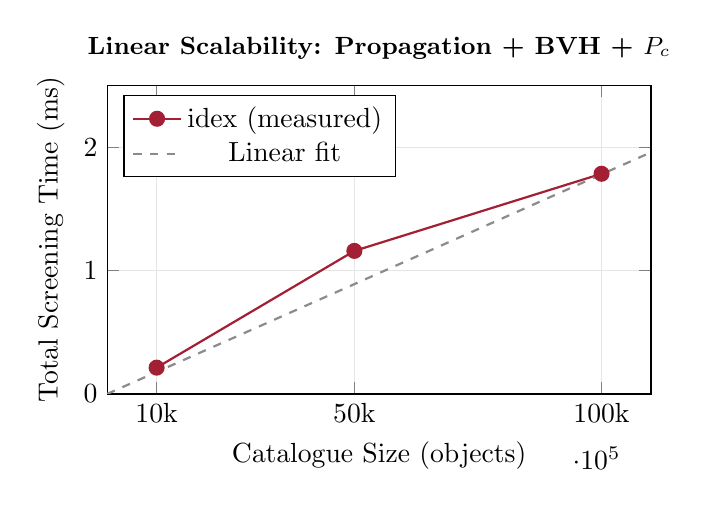
\begin{tikzpicture}
\begin{axis}[
    width=0.7\textwidth, height=5.5cm,
    xlabel={Catalogue Size (objects)},
    ylabel={Total Screening Time (ms)},
    grid=major, grid style={gray!20},
    xmin=0, xmax=110000, ymin=0, ymax=2.5,
    xtick={10000,50000,100000},
    xticklabels={10k,50k,100k},
    mark size=2.5pt,
    legend pos=north west,
    title={\textbf{Linear Scalability: Propagation + BVH + $P_c$}},
    title style={font=\small},
]
\addplot[color=mitred,mark=*,thick] coordinates {
    (10000, 0.213) (50000, 1.159) (100000, 1.784)
};
\addlegendentry{idex (measured)}
\addplot[color=mitgray,dashed,thick,domain=0:110000] {0.0000178*x};
\addlegendentry{Linear fit}
\end{axis}
\end{tikzpicture}
\caption{Empirical scalability of idex conjunction screening pipeline.
100k objects processed in 1.78\,ms (target: 45\,s). Memory: 3.1\,MB.}
\end{figure}

\textbf{Maturity status by component:}

\renewcommand{\arraystretch}{1.2}
\begin{tabularx}{\textwidth}{l Y c}
\toprule
\textbf{Component} & \textbf{Description} & \textbf{TRL} \\
\midrule
SGP4/HPOP/CR3BP Propagation  & Full perturbation model; validated vs.\ NORAD TLEs          & 5 \\
Swept-BVH + Foster--Alfano $P_c$ & Sub-2\,ms screening for 100k objects; CI-green              & 5 \\
3-Mode IMM Filter            & Ballistic/glide/manoeuvre; Bayesian mode adaptation          & 4 \\
Sliding SINDy Discovery      & Residual-targeted sparse regression; interpretable equations & 4 \\
gRPC/mTLS Server             & Ed25519 authentication; live WebSocket streaming             & 5 \\
DPHNO Neural Architecture    & Cholesky-enforced energy conservation; architecture frozen   & 3 \\
Conformal UQ                 & Distribution-free coverage certificates; integrated design   & 3 \\
ONNX Go Bridge               & Production ML-inference binding; Phase~1 integration target  & 2 \\
\bottomrule
\end{tabularx}

\pagebreak

% =============================================================================
\section{Capabilities \& Competencies}
% =============================================================================

\begin{itemize}
\item \textbf{Orbital Mechanics \& Astrodynamics:} Production-grade implementations
      of SGP4, HPOP (RKF4/5), CR3BP with state-transition matrix, symplectic
      integrators (Forest--Ruth, Yoshida-4), and initial orbit determination
      (Gauss method). Validated against NORAD TLEs.

\item \textbf{Physics-Informed Machine Learning:} Port-Hamiltonian neural
      operators with Cholesky-enforced dissipation guarantees. SINDy sparse
      regression for interpretable equation discovery. Conformal prediction
      for distribution-free uncertainty quantification.

\item \textbf{Systems Engineering (Go):} $>$150,000 lines of compiled Go with
      goroutine concurrency, embedded database persistence, gRPC/mTLS transport,
      and Ed25519 cryptographic signing. Multiple production binaries exceeding
      50\,MB total. CI/CD via GitHub Actions.

\item \textbf{Conjunction Analysis:} Foster--Alfano collision probability
      with Alfano 2005 error-function series, Monte Carlo surrogates,
      Mahalanobis-distance feature extraction, and dimensionless scaling
      for regime-invariant ML training.

\item \textbf{Hypersonic Threat Tracking:} 3-mode IMM filter with
      online Bayesian mode adaptation, free-energy-based adversarial intent
      scoring, and structured dynamic covariance propagation.

\item \textbf{Defence Domain Awareness:} Familiarity with ITAR/EAR/SCOMET
      compliance, iDEX SPRINT $\to$ ADITI $\to$ DAP Make-II procurement
      pathway, and Indian sensor network topology (Hanle, Mt Abu, NETRA,
      NavIC).
\end{itemize}

\vspace{2em}
\begin{center}
\rule{0.5\textwidth}{0.4pt}\\[0.8em]
{\small\textit{This document reflects the verified state of idex as of May 2026.
Live binaries, benchmark results, and end-to-end pipeline demonstrations
are available upon request under appropriate NDA. All proprietary algorithms,
source code, and trained model weights are privately held; full technical
disclosure is available under NDA/security clearance.}}
\end{center}

\vspace{1cm}
\begin{center}

\begin{tikzpicture}
  \fill[saffron]   (0,0) rectangle (5.3,0.10);
  \fill[white]     (5.3,0) rectangle (10.6,0.10);
  \fill[indiagreen](10.6,0) rectangle (15.9,0.10);
\end{tikzpicture}\\[0.4cm]
{\small\textcolor{mitgray}{\textit{Document generated for IAF ADITI 4.0 Challenge 24 submission}}}\\
{\small\textbf{\textcolor{mitred}{UBERMASCHINE PVT LTD}} \textbar\ All Rights Reserved}\\
{\small\textcolor{mitgray}{Classification: RESTRICTED --- For IAF Evaluation Only}}
\end{center}

\end{document}
